\chapter{Electronic Design}

\graphicspath{{./Figures/Electronic Design/}}
In this chapter, the details of the electronic design are presented.
Where it emphasizes the details of the components' technical specifications and the selection process.
In addition to the wiring tree of the electronic components and the PCB design,
The chapter also discusses the power management.


\begin{itemize}
	\item Overview of the chapter's focus.
	\item Emphasize the importance of electronic design in the context of the overall project.
\end{itemize}


\section{Design Objectives and Constraints}
\begin{itemize}
	\item Clearly define the objectives and goals for the electronic design
	\item Discuss any constraints such as power requirements, size limitations.
\end{itemize}
\section{Component Selection}
The component diagram is shown in figure \ref{fig:componentsdiagram} shows the different components and their relationship with each other.
The main components are the microcontroller, rassberry pi, the motors, Distance sensor, Camera, the battery.
%figure of the components digram
\begin{figure}[h]
	\centering
	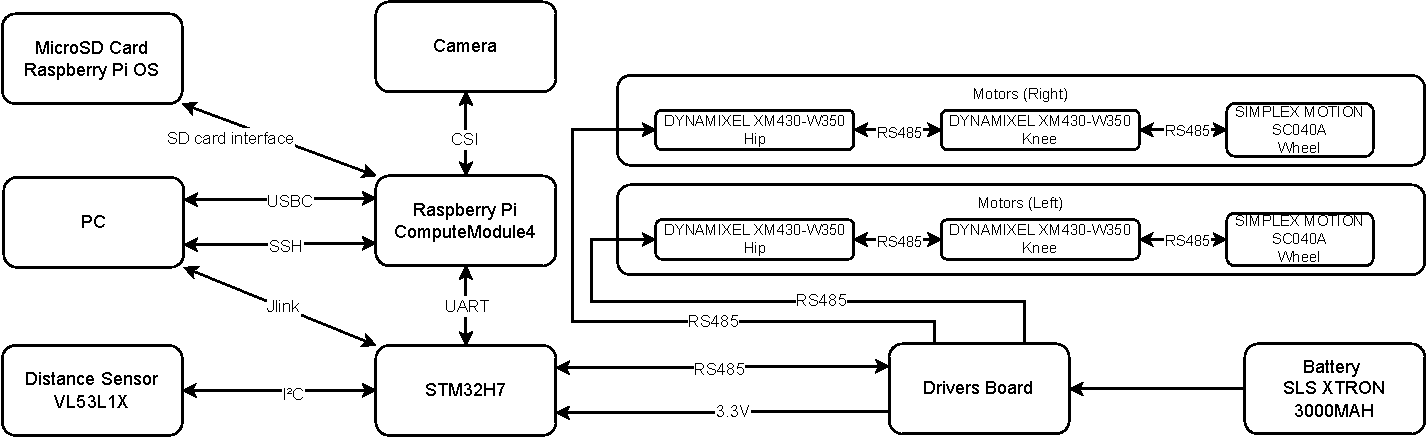
\includegraphics[width=1\linewidth]{Component_Diagram}
	%\includegraphics[width=0.5\linewidth]{Figures/Mechanical Design/Conceptual_Design}
	\caption[Components Diagram]{Components Diagram and there realationship with each other}
	\label{fig:componentsdiagram}
\end{figure}
\subsection{Hip and Knee Motors
%Details the selection process for key electronic components like microcontrollers,sensors, actuators, power supplies, etc.
The DYNAMIXEL XM430-W350 is chosen as a motor for the hip joint and the knee joint. The motor is chosen because it has a high torque to weight ratio and it has a high resolution of 4096 steps per revolution. The motor has a built-in driver and it can be controlled using a serial communication protocol. The motor has a built-in encoder that can be used to measure the position of the motor. The motor has a maximum torque of 3.5 Nm and a maximum speed of 46 RPM. The motor has a maximum current of 2.1 A and a maximum voltage of 12 V. The motor has a weight of 82 g and a size of 28.5 x 46.5 x 34 mm.
%figure of the DYNAMIXEL XM430-W350 motor
\begin{figure}[h]
	\centering
	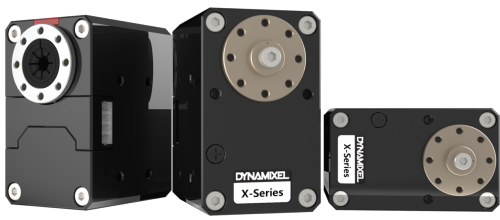
\includegraphics[width=0.5\linewidth]{DYNAMIXEL_XM430-W350}
	%\includegraphics[width=0.5\linewidth]{Figures/Mechanical Design/Conceptual_Design}
	\caption[DYNAMIXEL XM430-W350]{DYNAMIXEL XM430-W350}
	\label{fig:DYNAMIXEL_XM430-W350}
\end{figure}
%from the info on the website for SIMPLEX MOTION SC040A
%Continuous output of 120W and 280 mNm torque at 4000rpm
%Brushless outer rotor motor with peak torque of 800 mNm
%Integrated drive electronics with 4096 positions/revolution position sensor
%PID regulator for position or speed control with torque limit
%Ramp control of speed or position
%Protection features for current, torque, voltage and temperature
%Serial interface RS485 with Modbus RTU protocol
%CANOpen 301 interface
%Quadrature encoder input for application use
%Interface signals for step motor emulation (step/direction)
%Up to 8 digital inputs and 4 analog inputs
%4 digital outputs capable of 30V/1A, with pulse, PWM and RC Servo control modes.
%PC based software for setup and testing

The SIMPLEX MOTION SC040A is chosen as a motor for the wheels. The motor is chosen since it has a output of 120W and 280 mNm torque at 4000rpm. The motor has a built-in driver and it can be controlled using RS485 serial communication protocol. The motor has  position and speed control with torque limit. The motor has a maximum torque of 800 mNm.
%figure of the SIMPLEX MOTION SC040A motor
\begin{figure}[h]
	\centering
	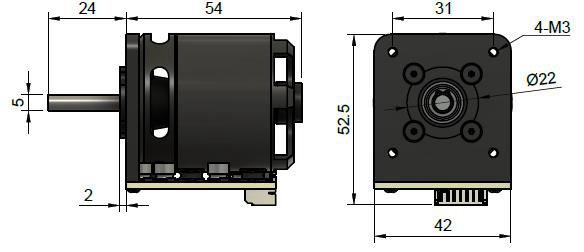
\includegraphics[width=0.5\linewidth]{SIMPLEX_MOTION_SC040A}
	%\includegraphics[width=0.5\linewidth]{Figures/Mechanical Design/Conceptual_Design}
	\caption[SIMPLEX MOTION SC040A]{SIMPLEX MOTION SC040A}
	\label{fig:SIMPLEX_MOTION_SC040A}
\end{figure}


%Rationale behind the choice of each component, focusing on specifications and performance requirements.

\section{Circuit Design}
%figure of the electronic design
\begin{figure}[h]
	\centering
	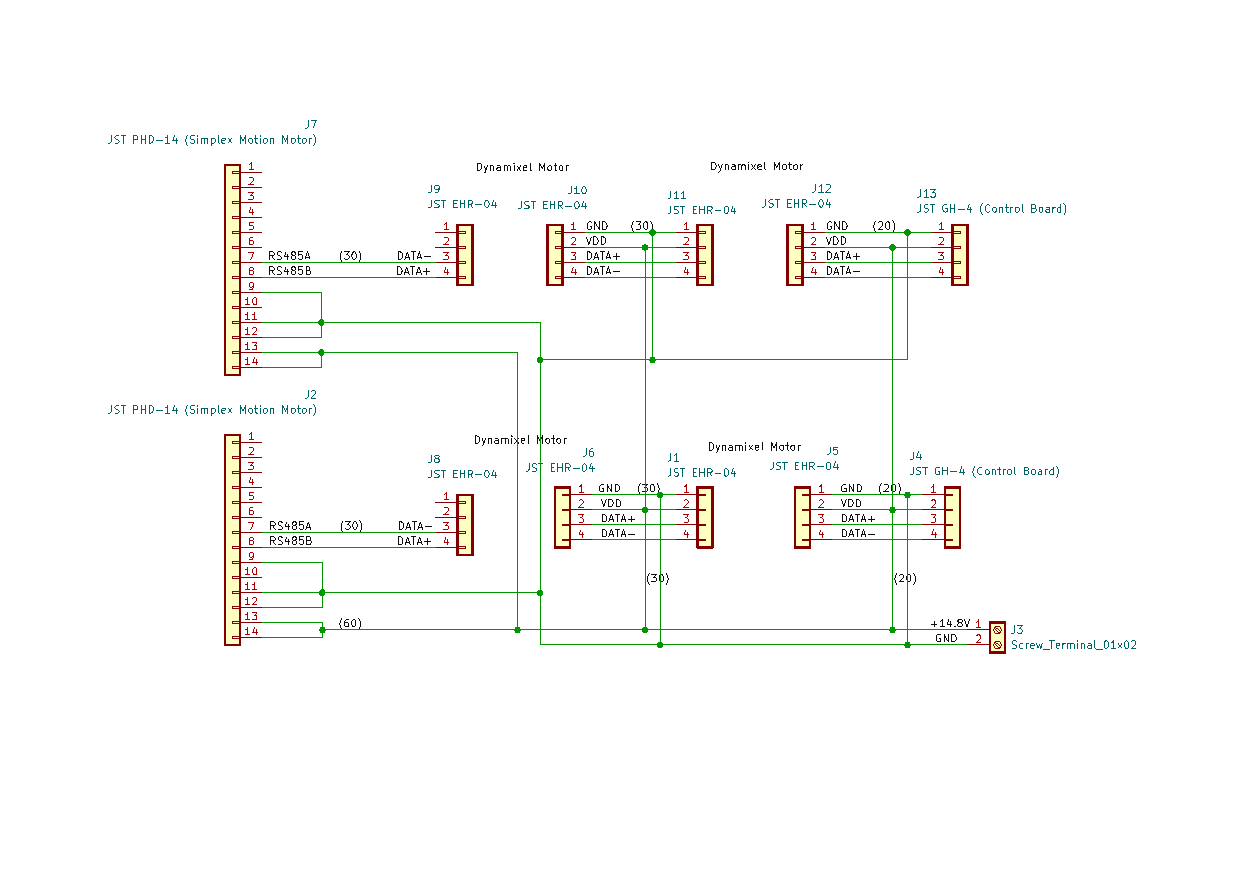
\includegraphics[width=1\linewidth]{Legged_TWIPR_Wiring_Tree}
	%\includegraphics[width=0.5\linewidth]{Figures/Mechanical Design/Conceptual_Design}
	\caption[ brakets for delectronic design second test ]{Electronic Design}
	\label{fig:electronicdesign}
\end{figure}
%expanation of the electronic design
The wiring tree of the electronic components is shown in figure \ref{fig:electronicdesign} where it shows the connection between the different components and the microcontroller.The first motor of each leg is connected to the microcontroller and the rest of the motors are connected in series to the first motor of using daisy chain connection. the motors have the drivers board intigrated so they only need the control signal comimg from the microcontroller.
\begin{itemize}
	\item Provide comprehensive information about the circuit design, including schematic diagrams.
	\item Explain the functionality and interaction of different circuit components.
	\item Discuss the design considerations for signal integrity, power distribution, and noise reduction.
\end{itemize}
\section{PCB (Printed Circuit Board) Design}
\begin{itemize}
	\item Describe the layout and design of any custom PCBs used in the project.
	\item Include information about PCB fabrication and assembly processes.
\end{itemize}
\section{Power Management}
\begin{itemize}
	\item Discuss how power is managed and distributed within the system.
	\item Include details on battery management, voltage regulation, and power efficiency considerations.
\end{itemize}